\documentclass[default]{subfiles}

\addbibresource{cite.bib}

\begin{document}

\selectlanguage{english}

\graphicspath{{image/}}

\udc{} % TODO
\pacs{} % TODO
\edn{} % TODO

\documentType{Review}

\title{Modern Methods of Non-invasive Determination of FFR Based on Computed Tomography Data}

\author[rudn]{Konstantin G. Leladze}
\author[rudn]{Larisa V. Alexandrova}

\address[rudn]{RUDN University, 6 Miklukho-Maklaya St, Moscow, 117198, Russian Federation}

\received{31}{12}{2025} % TODO
\revised{31}{12}{2025} % TODO
\accepted{31}{12}{2025} % TODO

\begin{authordescription}
    \authorfull[english]{Leladze, Konstantin G.}
    \authordegree[english]{Master's Degree in Computer Science}
    \authorpost[english]{PhD student of Department of
      Mathematical Modeling and Artificial Intelligence of  Peoples' Friendship University of Russia (RUDN University)}
    \email{1142230347@pfur.ru}
    \orcid{0009-0002-3023-9496}
\end{authordescription}

\begin{authordescription}
  \authorfull[english]{Alexandrova, Larisa V.}
  \authorpost[english]{
    Senior Lecturer at the Department of Mathematical Modeling and Artificial Intelligence of  Peoples'
    Friendship University of Russia (RUDN University)
  }
  \email{alexandrova-lv@rudn.ru}
  \orcid{0000-0002-5477-1551}
  \phone{+7(910)466-2375}
\end{authordescription}

\abstracts{
  This article provides a review of contemporary methods for constructing three-dimensional models of internal organs
  and blood vessels based on computed tomography (CT) imaging data in the context of non-invasive determination of
  fractional flow reserve (FFR). The study covers various algorithmic approaches aimed at improving the accuracy and
  reliability of reconstructing the surface geometry of internal organs and vessels. Key modern approaches, including
  segmentation algorithms, boundary detection methods, and machine learning techniques in image processing, are
  discussed.
}

\keywords{
  Fractional Flow Reserve (FFR), non-invasive imaging, computed tomography (CT), 3D reconstruction, image
  segmentation, coronary artery disease (CAD), machine learning
}
\alttitle{Современные методы неинвазивного определения ФРК на основании данных компьютерной томографии}

\altauthor[rudn]{К. Г. Леладзе}
\altauthor[rudn]{Л. В. Александрова}

\altaddress[rudn]{Российский университет дружбы народов, ул. Миклухо-Маклая, д.6, Москва, Россия, 117198}

\altabstracts{
  В данной статье представлен обзор современных методов построения трёхмерных моделей внутренних органов и сосудов на
  основании данных компьютерной томографии (КТ) в контексте задачи неинвазивного определения фракционного резервного
  кровотока (ФРК). Исследование охватывает различные алгоритмические подходы, применяемые для  повышения точности и
  надёжности реконструкции геометрии поверхности внутренних органов и сосудов. Рассмотрены ключевые современные
  подходы, включая алгоритмы сегментации, методы на основании детектирования границ и методы машинного обучения в
  обработке изображений.
}

\altkeywords{
  Фракционный резерв кровотока (ФРК), неинвазивная визуализация, компьютерная томография (КТ), трёхмерная
  реконструкция, сегментация изображений, ишемическая болезнь сердца (ИБС), машинное обучение
}

\maketitle

\section{Purpose of the Article}

The aim of this article is to provide a review of modern algorithmic approaches for constructing three-dimensional
models of internal organs and blood vessels based on computed tomography (CT) data in the context of non-invasive
fractional flow reserve (FFR) estimation, with a focus on segmentation methods, boundary detection techniques, and the
application of machine learning to improve the accuracy and reliability of geometric reconstruction.

\section{Introduction}

\label{sec:intro}

Non-invasive determination of fractional flow reserve (FFR) is essential for accurately assessing the condition of
coronary arteries without the need for invasive procedures. This approach enables the identification of stenoses that
may require treatment, thereby reducing the risk of complications and improving patient outcomes. FFR derived from
angiography serves as a valuable tool in decision-making for the diagnosis and treatment of coronary stenosis in
catheterization laboratories. This technology assists cardiologists in evaluating and managing moderate stenoses by
integrating both physiological and anatomical parameters of the coronary arteries.

Moreover, non-invasive methods reduce patient discomfort and stress, as they do not require catheter insertion into the
arteries. Ultimately, this facilitates earlier and safer detection of coronary artery disease. As a result,
non-invasive FFR estimation has become one of the most in-demand technologies in both domestic and global clinical
practice.

\section{Applicability of Non-invasive Approaches for FFR Determination}

Study \cite{lu2017ffr} compares non-invasive FFR estimation methods based on CT imaging with invasive techniques,
investigating whether combining the two improves the predictive accuracy for various conditions such as stenosis and
ischemia. The authors conclude that incorporating data obtained through modeling leads to more accurate disease
prediction, indicating the positive impact of non-invasive FFR assessment in clinical practice.

Similar findings are reported in publications \cite{patel2020advance, villines2020advance, norgaard2019ctffr,
agasthi2018meta, douglas_2009, vanrosendael_2020, jonas_2025, jensen_2012}. Specifically, study
\cite{patel2020advance} demonstrates significantly lower mortality in the group of patients with negative non-invasive
FFR results compared to those with positive results. Meanwhile, publication \cite{agasthi2018meta, rao_2023} shows that
the use of non-invasive FFR methods yields high diagnostic accuracy and performs well in comparison to invasive FFR in
assessing the significance of coronary stenotic lesions. These studies emphasize that non-invasive FFR techniques are
still evolving and require further refinement and clinical validation before widespread clinical implementation.

\section{Methods of Non-invasive FFR Determination}

Traditionally, non-invasive FFR estimation relies on various vessel segmentation algorithms \cite{pal1993segmentation},
which are used to build a blood flow model and perform fluid dynamics simulations within the reconstructed geometry
using specialized software such as Ansys.

One of the main types of segmentation algorithms is the family of region-growing algorithms. These take a series of CT
images and a set of initial coordinates (seeds) as input and expand regions from these seed points. The output is
typically a set of voxels forming the region of interest \cite{revol1997regiongrow}. Due to the need for manual seed
selection, these algorithms are considered semi-automatic. They are commonly used to segment internal organs and their
components. For example, study \cite{bajaj2015heart} describes the process of constructing a patient-specific heart
model based on high-resolution CT data. The publication demonstrates the possibility of segmenting the region of
interest into separate components such as the heart, blood vessels, and others. A similar approach is also described
and applied in \cite{mcqueen2005heart}.

Some studies are limited to constructing one-dimensional vessel models directly from CT data. Such an approach is
presented in \cite{carson2019benchmark}, but its applicability is limited due to the inability to account for certain
individual anatomical features or the presence of plaques in the vessels, as explicitly noted in the study. Moreover,
according to publication \cite{gamage2022octffr}, taking into account features like vessel branching is highly
desirable, as it significantly affects the simulation results.

Undoubtedly, constructing a more precise 3D model of the vascular system improves the accuracy of simulations and FFR
estimation. Consequently, such technologies are in high demand and have become widespread.

In addition, boundary detection-based algorithms are also employed. Study \cite{ecabert2011heart} proposes a method for
constructing a model of the heart and its adjacent vascular system using a parameterized boundary detection algorithm.
The proposed method begins segmentation from an initial state based on an idealized, patient-averaged heart model and
iteratively converges to a state that represents the individual geometry of a specific patient’s heart. The transition
from one state to the next is performed so as to optimize a predefined quality functional. The study also includes a
validation phase that assesses the accuracy and quality of heart segmentation. Based on tests on data from three
patients and comparisons between automatically generated and manually created segmentations, the authors claim that
their approach is sufficiently accurate for practical use and can facilitate and accelerate quantitative analysis of
CT data for the diagnosis and treatment of cardiovascular diseases.

A method for constructing a three-dimensional region by "inflating" a deformable body is described in study
\cite{mcinerney1995fem}. The authors employ a parameterized energy functional that models the behavior of the elastic
surface of the expanding body, along with a system of differential equations that governs the process of filling the
region of interest, which is bounded by the walls of internal organs or blood vessels. Laplace equations are used to
describe the behavior of the body under the influence of both the expanding force and surface tension forces. The
system is solved using a finite element mesh specifically designed for the task, consisting of triangular elements in
the space $\mathbf{C}^1$.

\begin{figure}[H]
    \centering
    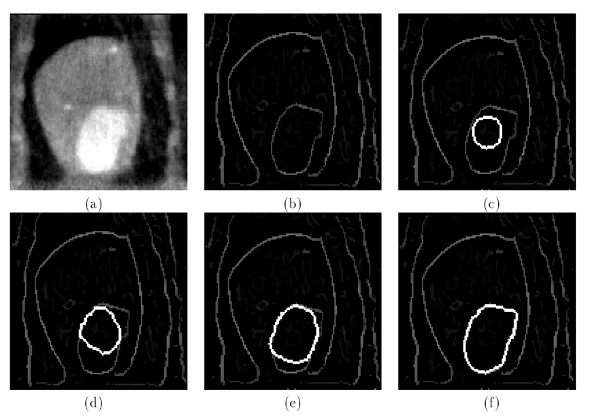
\includegraphics[width=0.7\textwidth]{image/pic1.png}
    \caption{The process of filling the region of interest with a deformable body \cite{ mcinerney1995fem, mcinerney2002deformable, mcinerney1996deformable, terzopoulos1997deformable, mcinerney1999topology}}
\end{figure}

Another method involves the interpolation of the boundaries of the heart and blood vessels using splines, resulting in
a smooth surface that segments the region of interest \cite{ecabert2008automatic}. Compared to polygonal models, such a
representation may be more suitable for simulating fluid flow for FFR estimation, as it allows for more precise and
interactive control over the generation of the finite element mesh. This, in theory, can lead to greater accuracy of
the simulation results \cite{morris_2013, fluids_2019, marcinno_2025}.

The algorithm described in publication \cite{lu2020vessels} enables vessel geometry reconstruction by first generating
an intermediate one-dimensional structure, similar to the approach in study \cite{carson2019benchmark}. The central
lines of the vessels are constructed first, and then the vessel walls are reconstructed based on individual anatomical
features using Frenet formulas. The output of the algorithm is a three-dimensional vessel model with a smooth surface,
which can be used to run simulations and model blood flow dynamics.

Such reconstruction methods are particularly valuable in the context of patient-specific modeling, where anatomical
variability plays a critical role in both diagnosis and treatment planning \cite{chakshu_2022}. Unlike generic or
population-based models, individualized vessel reconstructions account for the unique topological and morphological
features of a patient's vascular network, including curvature, bifurcations, and local variations in diameter. These
parameters are essential for achieving accurate hemodynamic simulations, especially when calculating pressure gradients
for non-invasive FFR estimation \cite{yu_2022}. Furthermore, the use of Frenet frames to reconstruct vessel walls based
on extracted centerlines allows for the generation of smooth and anatomically consistent geometries, which are
well-suited for finite element meshing and subsequent computational fluid dynamics (CFD) analysis
\cite{csippa_2021_decomposition}. This approach not only enhances the physiological relevance of simulations but also
reduces numerical instabilities during flow modeling, thereby improving the robustness and reliability of diagnostic
predictions \cite{decroocq_2023}.


\begin{figure}[H]
  \centering
  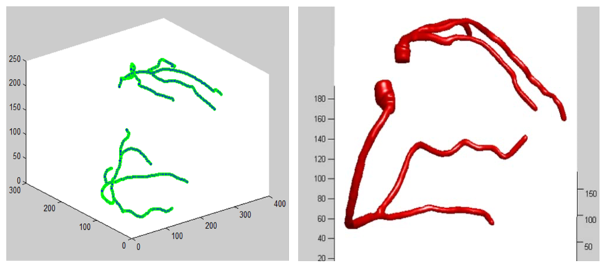
\includegraphics[width=0.7\textwidth]{image/pic2.png}
  \caption{Centerline of the vessels and their reconstructed geometry \cite{lu2020vessels}}
\end{figure}

Recently, convolutional neural network (CNN)-based approaches have also been used for reconstructing the geometry of
internal organs and blood vessels and building their three-dimensional models. For instance, the U-net model
\cite{ronneberger2015unet}, specifically developed for biomedical image segmentation tasks, is applied in study
\cite{ramakrishnan2023vessels}. The study compares the segmentation results produced by U-net with those of a Ground
Truth algorithm that relies on manual preprocessing, and concludes that U-net—and deep learning in general—shows high
applicability and significant potential for medical image segmentation tasks.

\begin{figure}[H]
    \centering
    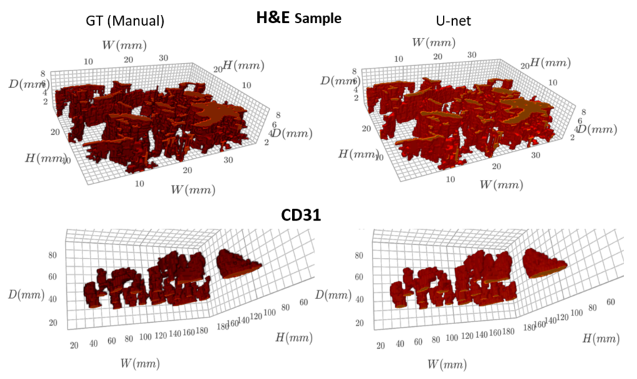
\includegraphics[width=0.7\textwidth]{image/pic3.png}
    \caption{Comparison of segmentation results using the GT algorithm and U-net
    \cite{ramakrishnan2023vessels, kohl_2019}}
\end{figure}

Study \cite{arefinia2024deepffr} presents a fast, end-to-end, and fully automated method for determining FFR using a
convolutional neural network (CNN) architecture, transfer learning, and a pre-trained DenseNet169 model to estimate FFR
values from angiographic images. The model architecture consists of feature extraction and classification layers, with
cross-entropy used as the loss function \cite{arefinia_2024}. A distinctive feature of this approach is the absence of
a vessel geometry reconstruction stage — the model directly takes input images and outputs the FFR value
\cite{wang_2019, mineo_2024}.

\begin{figure}[H]
    \centering
    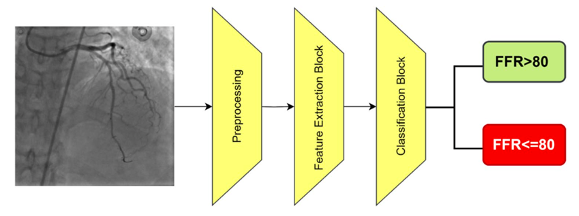
\includegraphics[width=0.7\textwidth]{image/pic4.png}
    \caption{Architecture of the proposed model \cite{arefinia2024deepffr}}
\end{figure}

\section{Current Results}

The review study \cite{khav2020ctffr} examines the progress of technologies and methods for non-invasive FFR estimation
as of 2020. The authors analyze the historical development of non-invasive FFR algorithms and summarize the current
achievements in the field.

\begin{figure}[H]
    \centering
    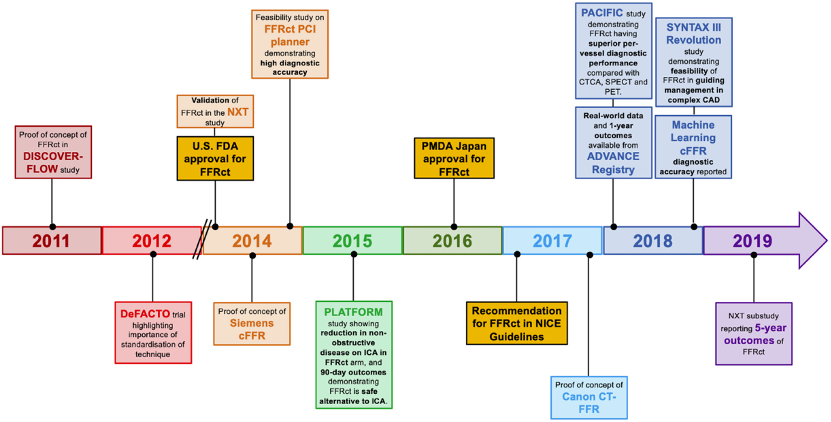
\includegraphics[width=0.7\textwidth]{image/pic5.png}
    \caption{History of non-invasive FFR (as of 2020) \cite{khav2020ctffr}}
\end{figure}

The researchers highlight the following findings: \newline

\begin{itemize}
\item Diagnostic accuracy: CT-based FFR has demonstrated high accuracy in diagnosing coronary artery disease,
comparable to invasive methods. Studies such as DISCOVER-FLOW, DeFACTO, and NXT have shown that non-invasive FFR
correlates strongly with invasive FFR and outperforms standard CT coronary angiography (CTCA) in diagnostic
performance \cite{debruyne_2012, bjarne_2014}.

\item Clinical outcomes: Non-invasive FFR allows for accurate identification of hemodynamically significant stenoses,
which is essential for decision-making regarding revascularization procedures (e.g., stenting). This helps avoid
unnecessary interventions in patients with non-critical stenoses \cite{morris_2013, belle_2018, chen_2019, cimen_2014}.

\item Advantages over invasive methods: Non-invasive techniques eliminate the risks associated with surgical procedures
and reduce patient discomfort \cite{mintz_2015, koo_2011}.

\item Practical clinical application: Integrating non-invasive FFR into clinical practice can enhance the diagnosis and
treatment of patients suspected of having coronary artery disease, reducing both diagnostic time and costs
\cite{asch_2015, gloekler_2014, dweck_2019}.

\item Future development: The authors emphasize the need for further large-scale studies to validate the diagnostic
effectiveness and safety of non-invasive FFR methods in routine clinical use.
\end{itemize}

\section{Conclusion}

This article has reviewed modern algorithmic approaches to the non-invasive determination of fractional flow reserve
(FFR) based on computed tomography data. The discussed methods—ranging from classical segmentation algorithms and
boundary detection techniques to deep learning-based models—demonstrate significant potential for improving the
accuracy and efficiency of FFR estimation. Non-invasive FFR provides a clinically valuable alternative to invasive
procedures, offering reduced risk, greater patient comfort, and strong diagnostic performance. While current results
are promising, further development and large-scale clinical validation are needed to ensure the reliability and
integration of these technologies into routine medical practice \cite{zhang_2025, }.

\section{Future Work}

Future research should focus on improving the accuracy and generalizability of non-invasive FFR estimation methods,
particularly those based on deep learning \cite{becker_2024, zhang_2025}. Expanding training datasets with diverse
clinical cases and CT scan protocols will enhance model robustness.

Further efforts are needed to develop fully automated and clinically integrable pipelines that combine segmentation,
modeling, and FFR calculation. Real-world validation on larger cohorts is essential to confirm diagnostic reliability
and assess long-term clinical impact.

Additionally, incorporating supplementary physiological parameters, such as myocardial perfusion or vessel wall
characteristics, may provide a more comprehensive and personalized evaluation of coronary artery disease.

\putbib[cite]

\makealttitle

\end{document}
